%   Filename    : chapter_4.tex 
\chapter{Results and Discussions/Analyses}
%This chapter  presents the results or  the system  of your SP.  Include screenshots, tables, or graphs and provide the discussion of results.
This chapter discusses the results and analysis of the study. As specified, the study focuses on building an animal rescue system that implements gamification and login features for the Aklan Animal Rescue and Rehabilitation Center in Kalibo, Aklan. 

\section{Results}

The state of the current web-based systems of animal rescue centers are straightforward
and simple. It is important to make it as user-friendly as possible so that
it would be easier for the users to engage in the system. But simplicity does
not always mean the more users would engage on it. Gamification integrates the
“human” to the system and is considered in designing that motivates more
users to take part in using the system.

There are general ways in finding out what motivates the user of an animal
rescue center,the researchers used that motivation to drive the users to do certain actions they would not normally do. The specific motivation for a web-based animal
rescue system that the researchers used is a virtual pet that evolves when it will reach a certain
level. The way to gain experience points to level up is by doing transactions in the animal rescue system like donating, adopting, and volunteering.

%Logo
\subsection{Logo}
\begin{figure}[h]              
	\centering                    
	
\includegraphics[width=13cm]{logo.png}  
	\caption{Rescue Pets Logo}
	\label{fig:disneystock}
	
\end{figure}

\newpage
\subsection{Sign-up Page}

\begin{figure}[h]              
	\centering                    
	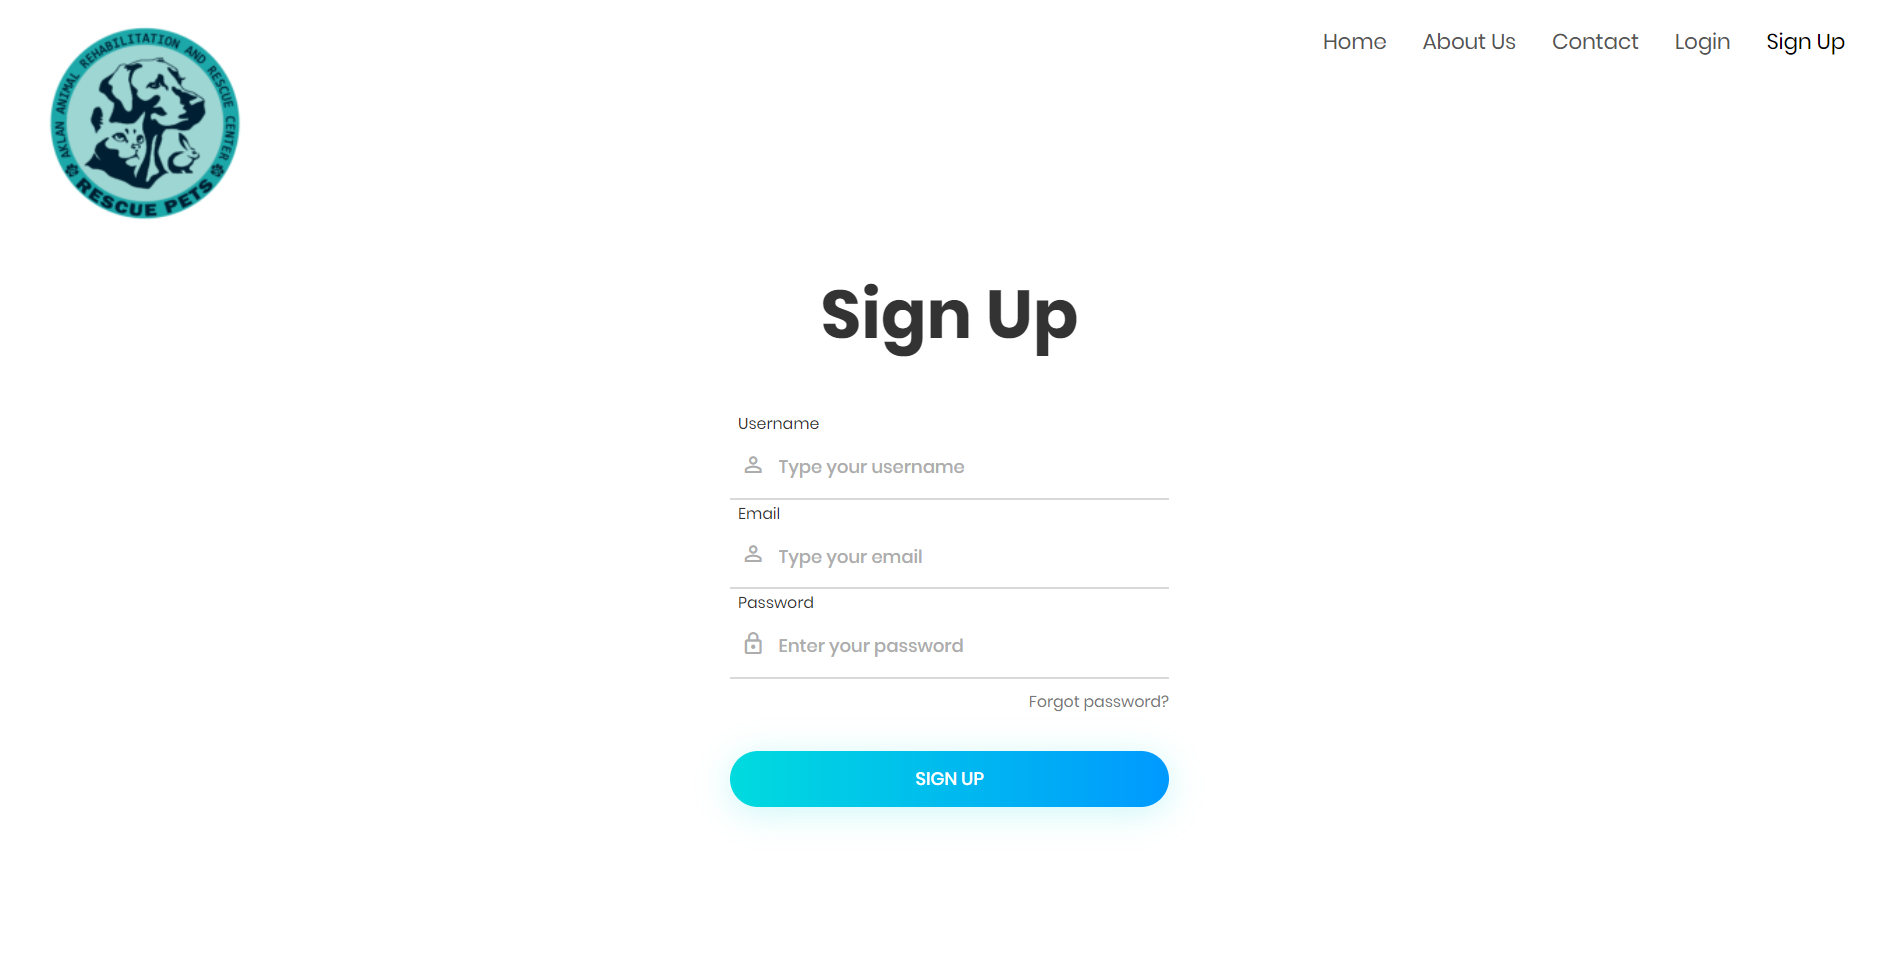
\includegraphics[width=13cm]{SignUpPage.png}  
	\caption{Sign-Up Page}
	\label{fig:disneystock}
		
\end{figure}

\begin{figure}[h]              
	\centering                    
	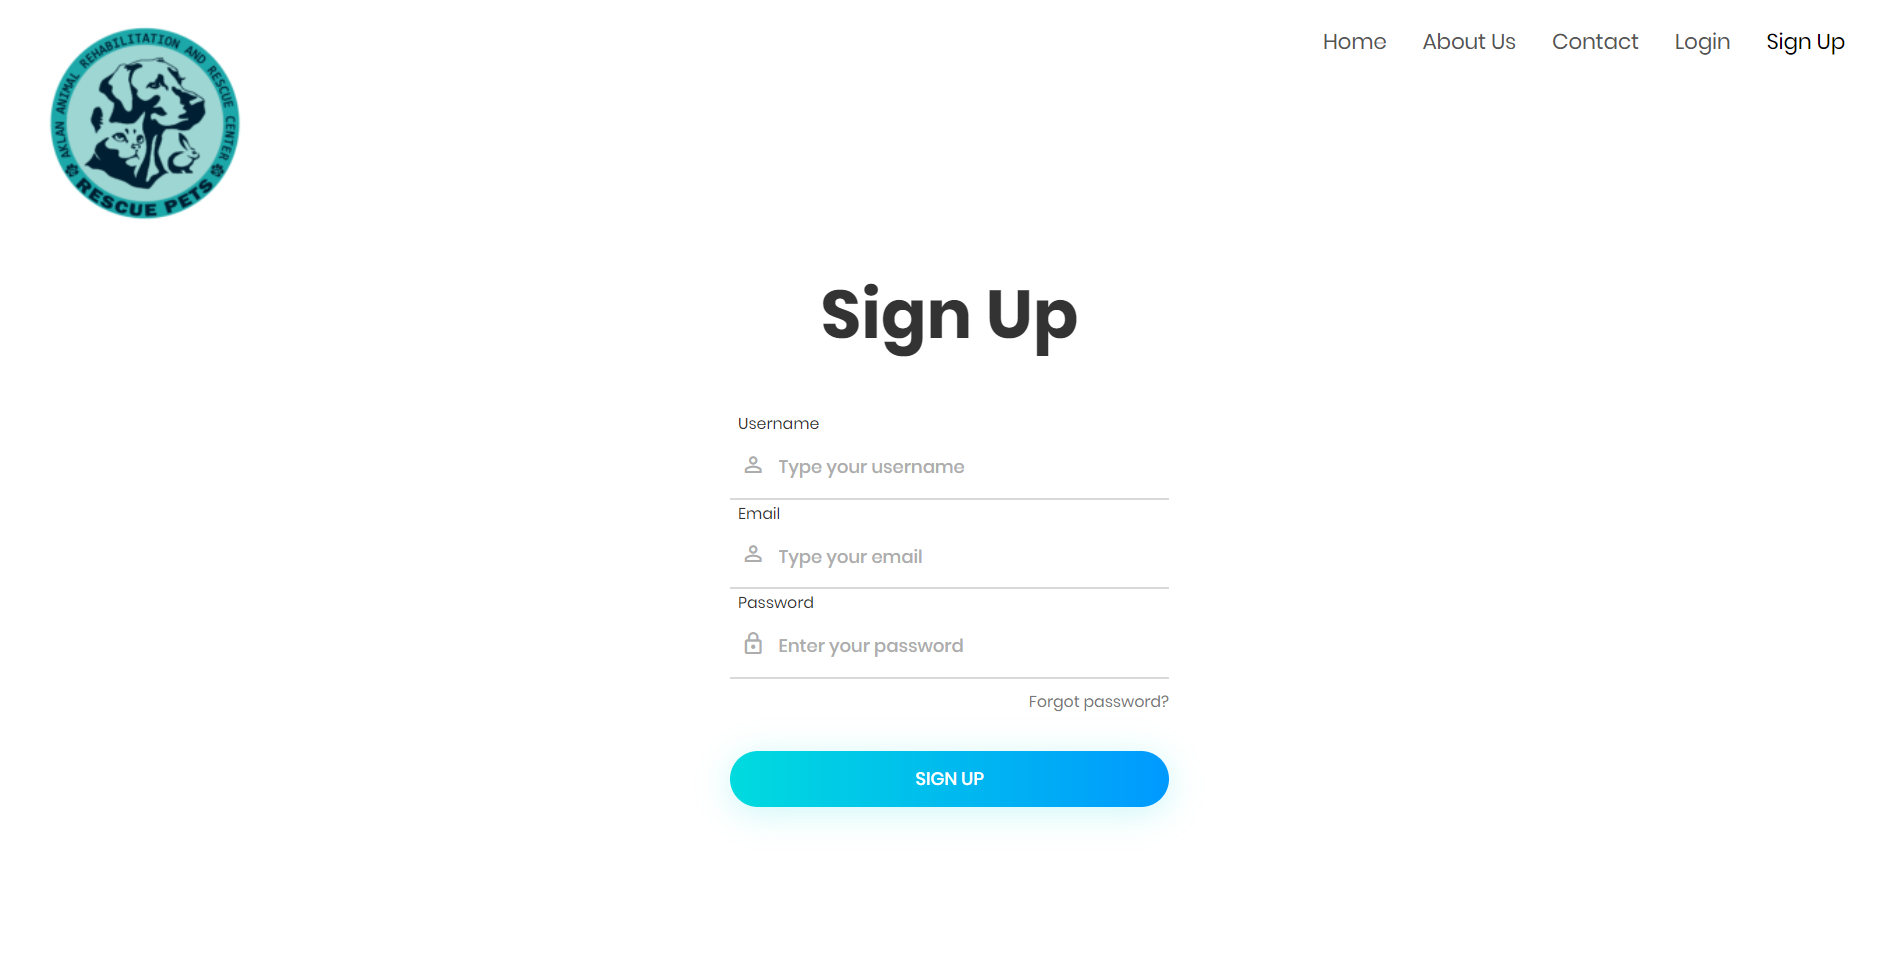
\includegraphics[width=13cm]{SignUpPage1.png}  
	\caption{Sign-Up Form}
	\label{fig:disneystock}
	
\end{figure}

\newpage
\subsection{Login Page}

\begin{figure}[h]                
	\centering                  
	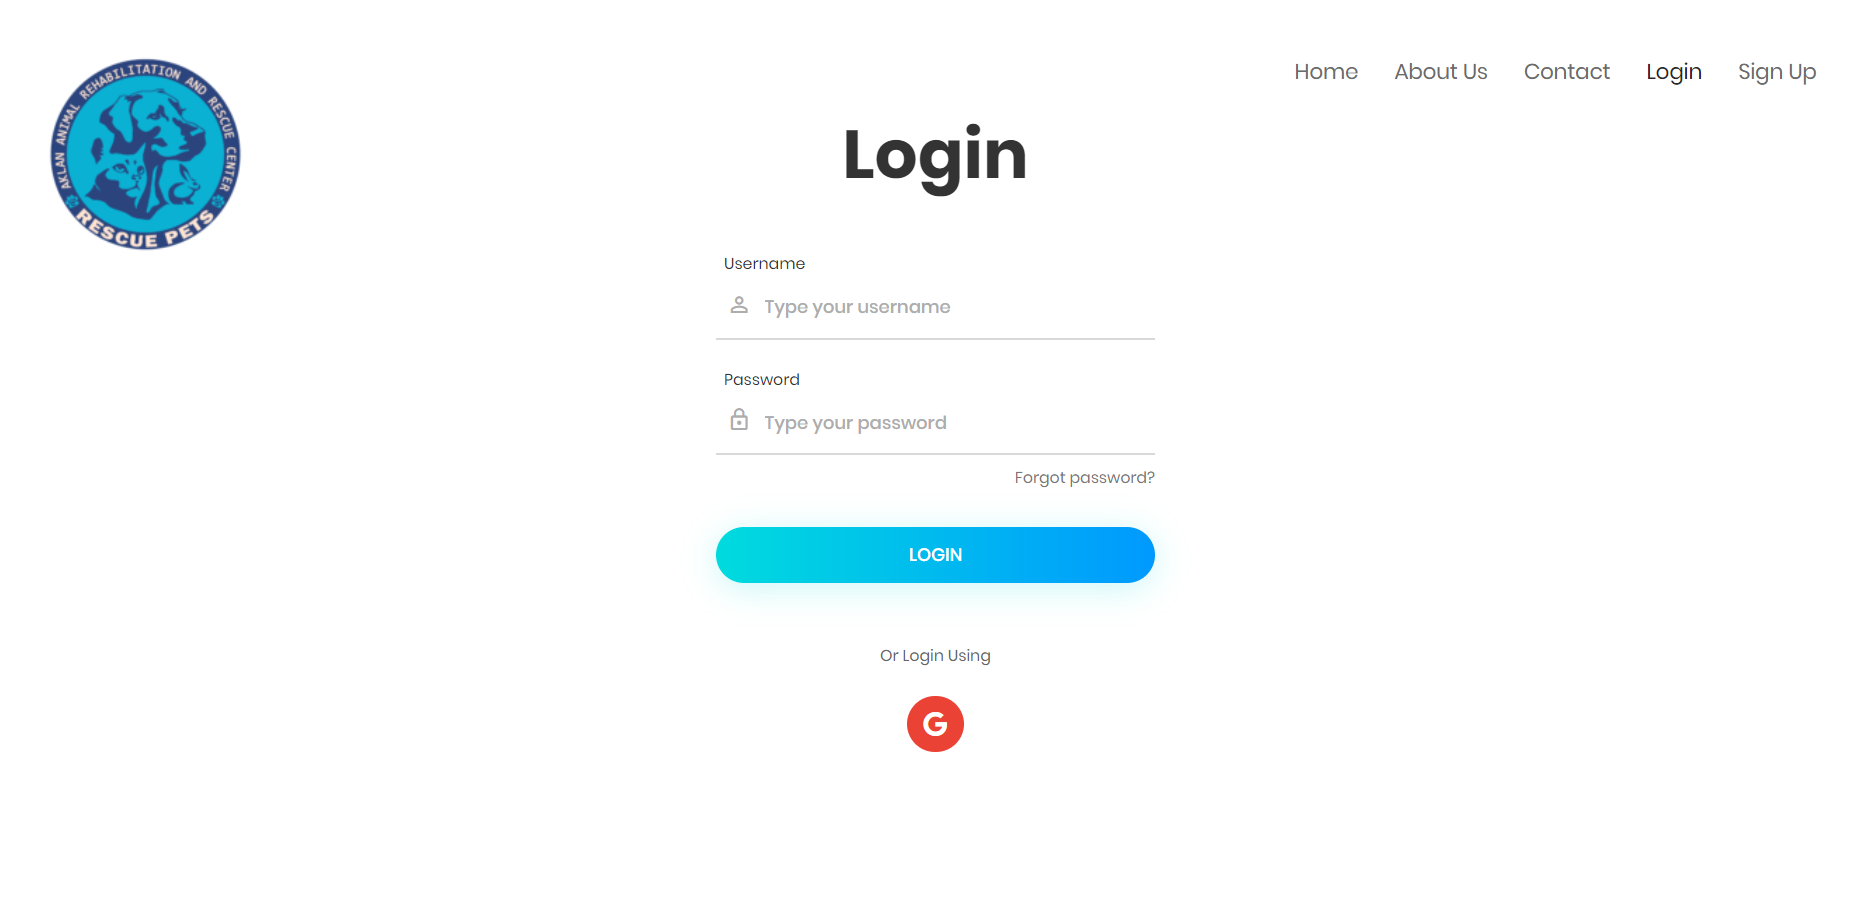
\includegraphics[width=15cm]{LoginPage.png}    
	\caption{The Login Page}
	\label{fig:disneystock}
\end{figure}

\subsection{Home Page}

\begin{figure}[h]
	\centering                    
	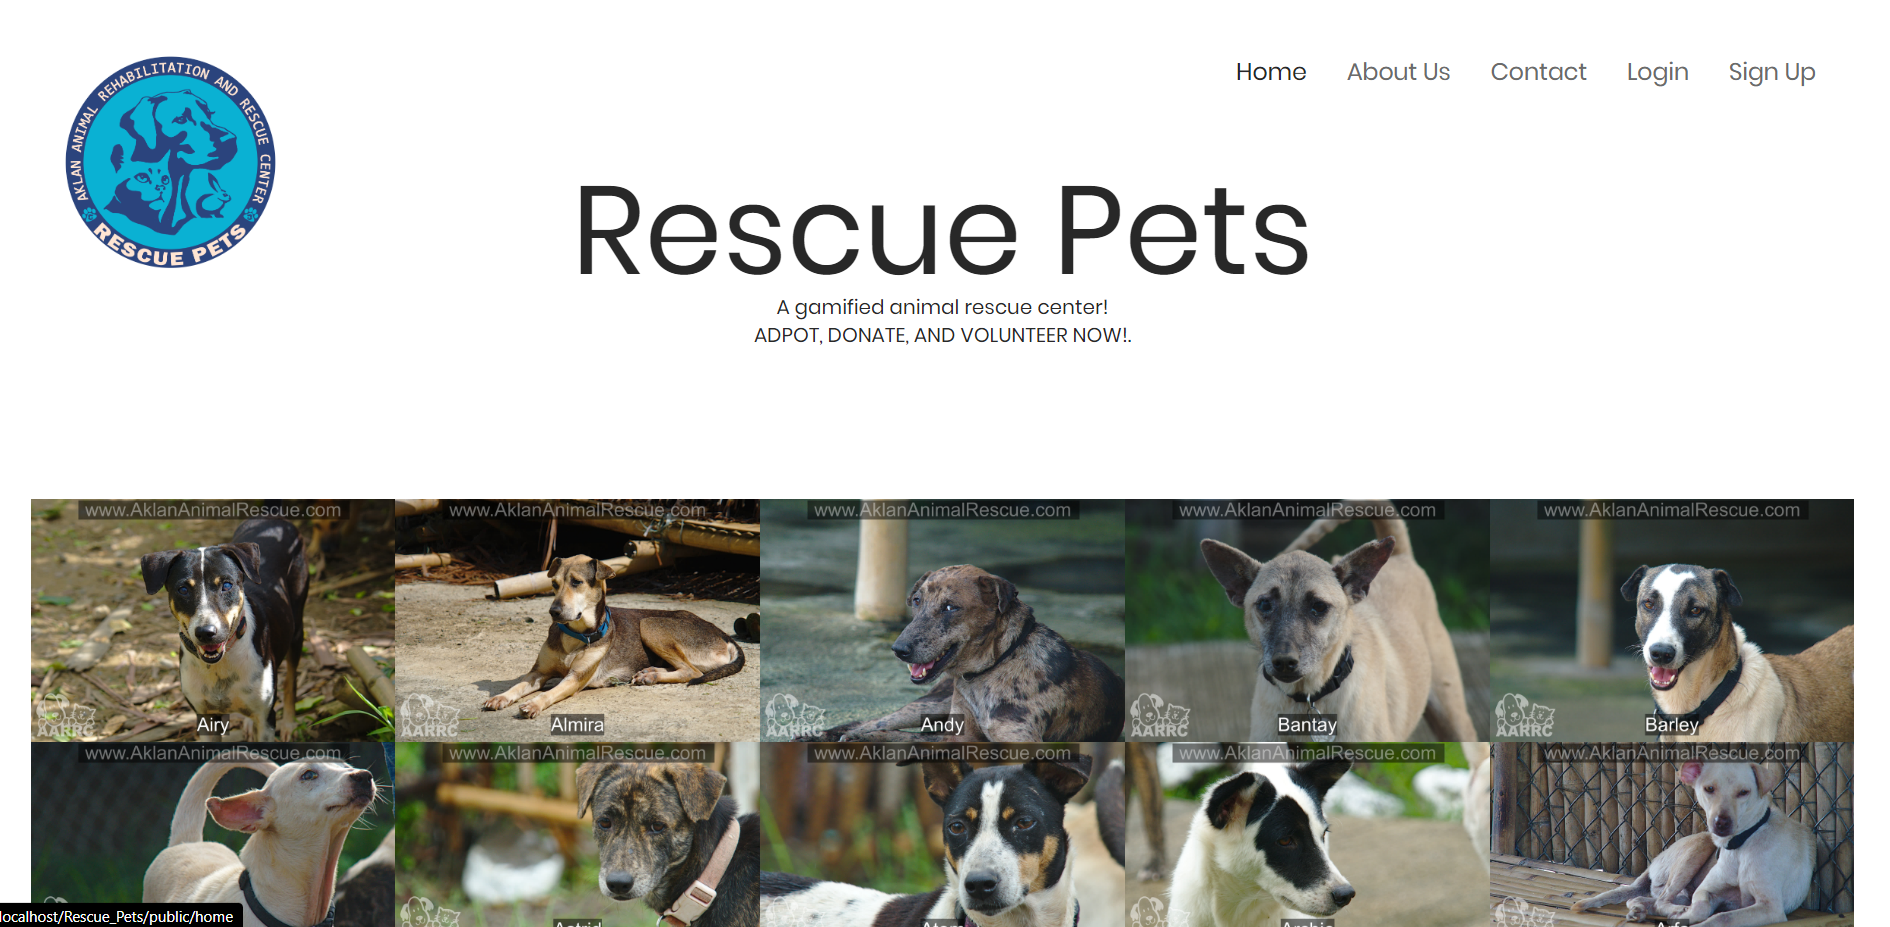
\includegraphics[width=13cm]{HomePage.png}       
	\caption{Home Page}
	\label{fig:disneystock}
\end{figure}

\newpage
\subsection{Information Page}

\begin{figure}[h]                
	\centering                   
	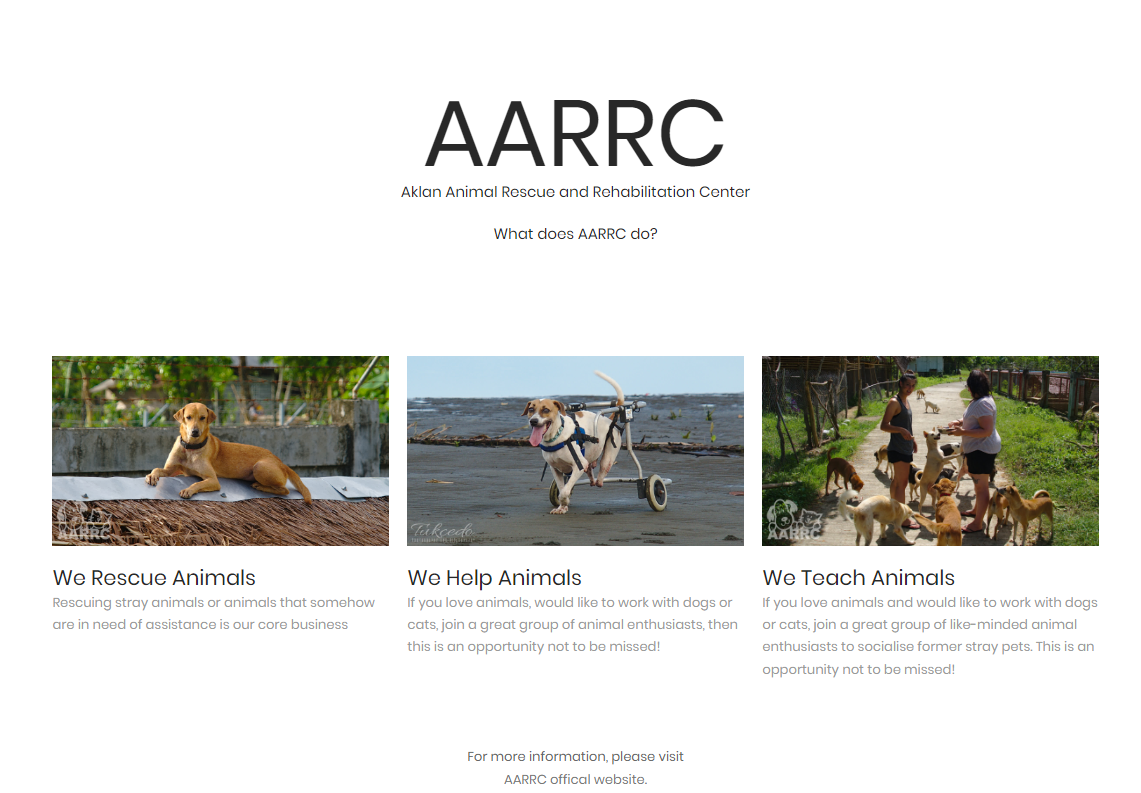
\includegraphics[width=13cm]{AboutUs.png}      
	\caption{About Aklan Animal Rehabilitation and Rescue Center}
	\label{fig:disneystock}
\end{figure}

\begin{figure}[h]                
	\centering                   
	
\includegraphics[width=13cm]{AboutUs1.png}      
	\caption{About Aklan Animal Rehabilitation and Rescue Center}
	\label{fig:disneystock}
\end{figure}

\newpage
\subsection{Contact Page}

\begin{figure}[h]                
	\centering                   
	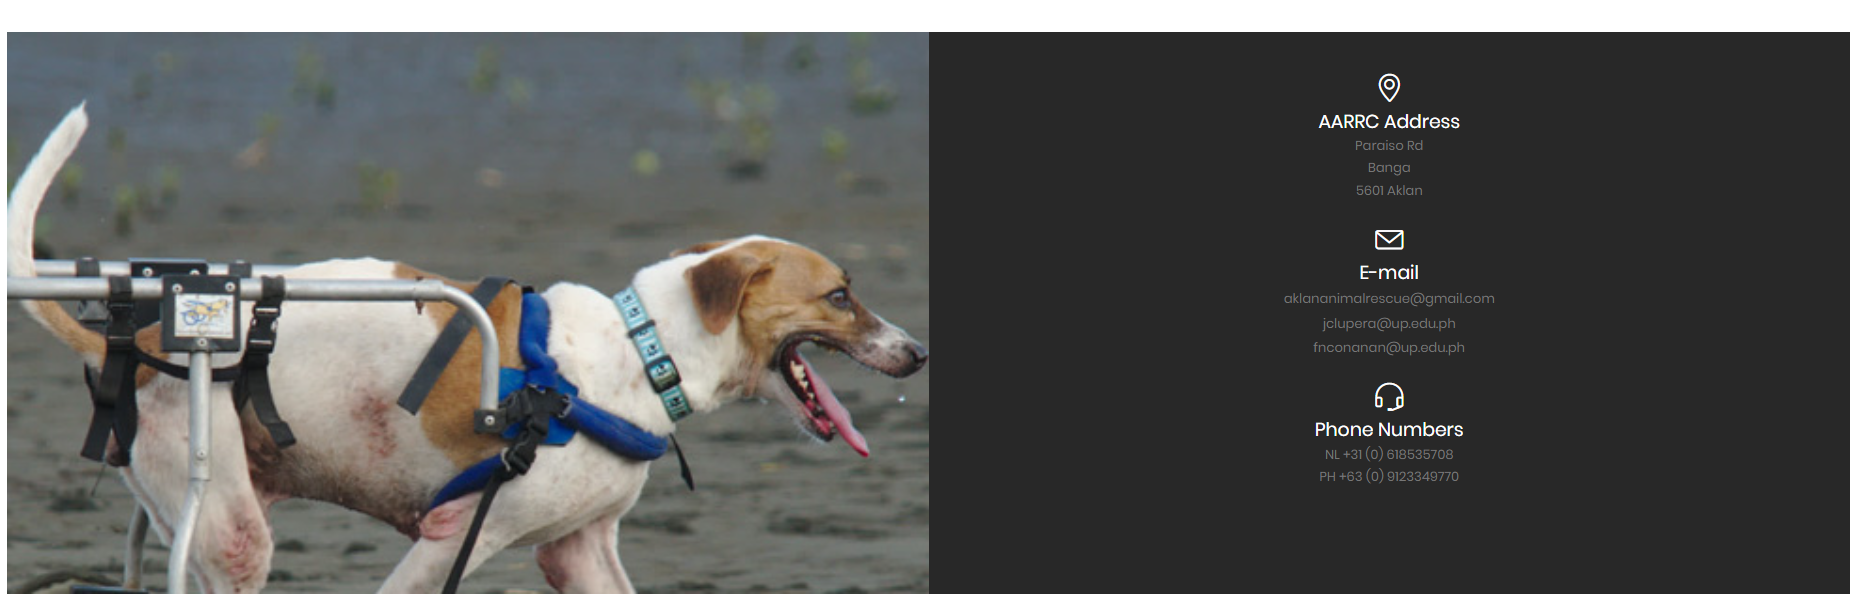
\includegraphics[width=13cm]{ContactPage.png}      
	\caption{Contact Us}
	\label{fig:disneystock}
\end{figure}

\subsection{Profile Page}

\begin{figure}[h]                
	\centering                   
	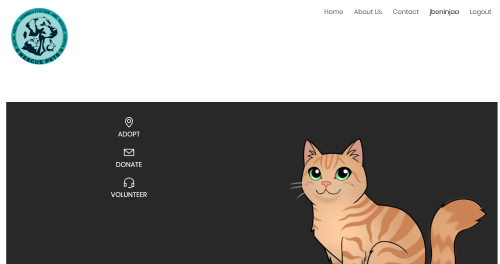
\includegraphics[width=13cm]{ProfilePage.png}      
	\caption{Profile Page}
	\label{fig:disneystock}
\end{figure}

\newpage
\subsection{Footer}

\begin{figure}[h]                
	\centering                   
	\includegraphics[width=15cm]{footer.png}      
	\caption{System Footer}
	\label{fig:disneystock}
\end{figure}

\subsection{Navigation Bar}
\begin{figure}[h]                
	\centering                   
	
\includegraphics[width=15cm]{NavigationBar.png}    
	\caption{Navigation Bar}
	\label{fig:disneystock}
\end{figure}

\newpage
\subsection{Virtual Pets}
\begin{figure}[h]                
	\centering                   
	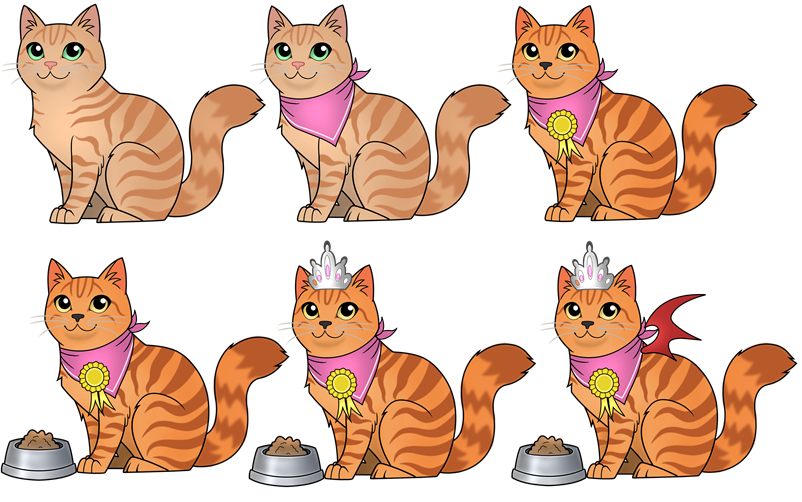
\includegraphics[width=6cm]{Cat.png}    
	\caption{Cat (transition from upper-left to lower right)}
	\label{fig:disneystock}
\end{figure}

\begin{figure}[h]                
	\centering                   
	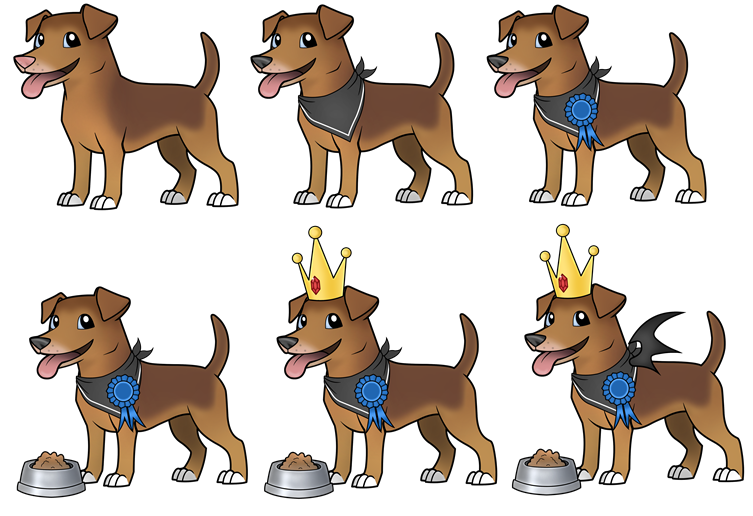
\includegraphics[width=6cm]{Dog.png}    
	\caption{Dog (transition from upper-left to lower right)}
	\label{fig:disneystock}
\end{figure}

\begin{figure}[h]                
	\centering                   
	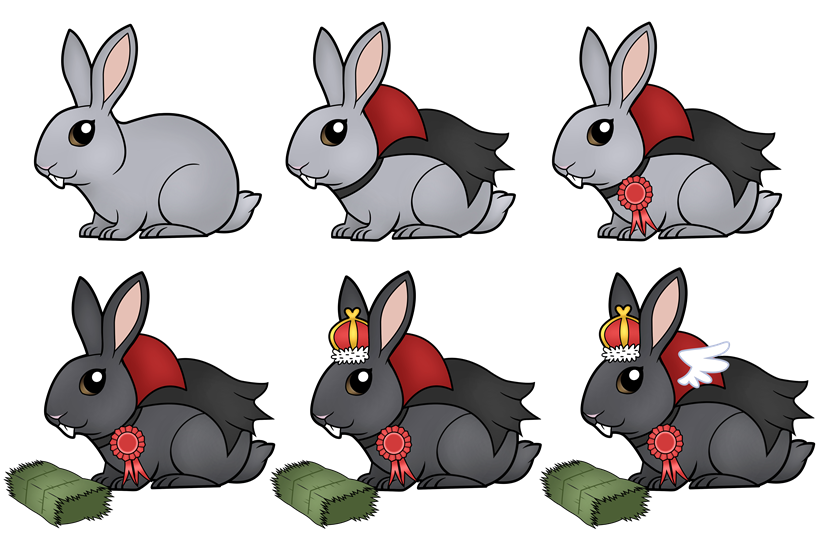
\includegraphics[width=6cm]{Rabbit.png}    
	\caption{Rabbit (transition from upper-left to lower right)}
	\label{fig:disneystock}
\end{figure}



